\documentclass{article}
\usepackage{amssymb}
\usepackage{geometry}
\usepackage{graphicx}

\geometry{letterpaper, margin=1in}
\title{Machine-Learning Methodology to Mitigate Ground Clutter in the 
GPM DPR observations}
\author{Mircea Grecu, Gerald M. Heymsfield, Stephen Nichols, Steven Lang, \and William S. Olson}
\begin{document}
\maketitle
\section*{Introduction}
In radar meteorology, the echo originating in power emitted by the radar
and reflected by the ground is called ground clutter. The ground 
clutter is a significant problem for the GPM DPR observations. 

\subsection*{Facts}
\begin{itemize}
    \item
      When plotted relative to the 0C isotherm Ku-band reflectivity profiles
      characterized by different freezing levels exhibit similar
      distributions.
    \item
      Same is true for precipitation, although some intensity differences
      are apparent. The intensity differences might be caused by different
      initial R-Dm relationships.
    \item
      Precipitation rates exhibit trends with range. Consequently,
      estimating the surface precipitation rate by setting it equal to the
      precipitation rate in the lowest clutter-free bin results in
      underestimation.
    %% include image
    
    \end{itemize}
    \begin{figure}[h]
        \centering
        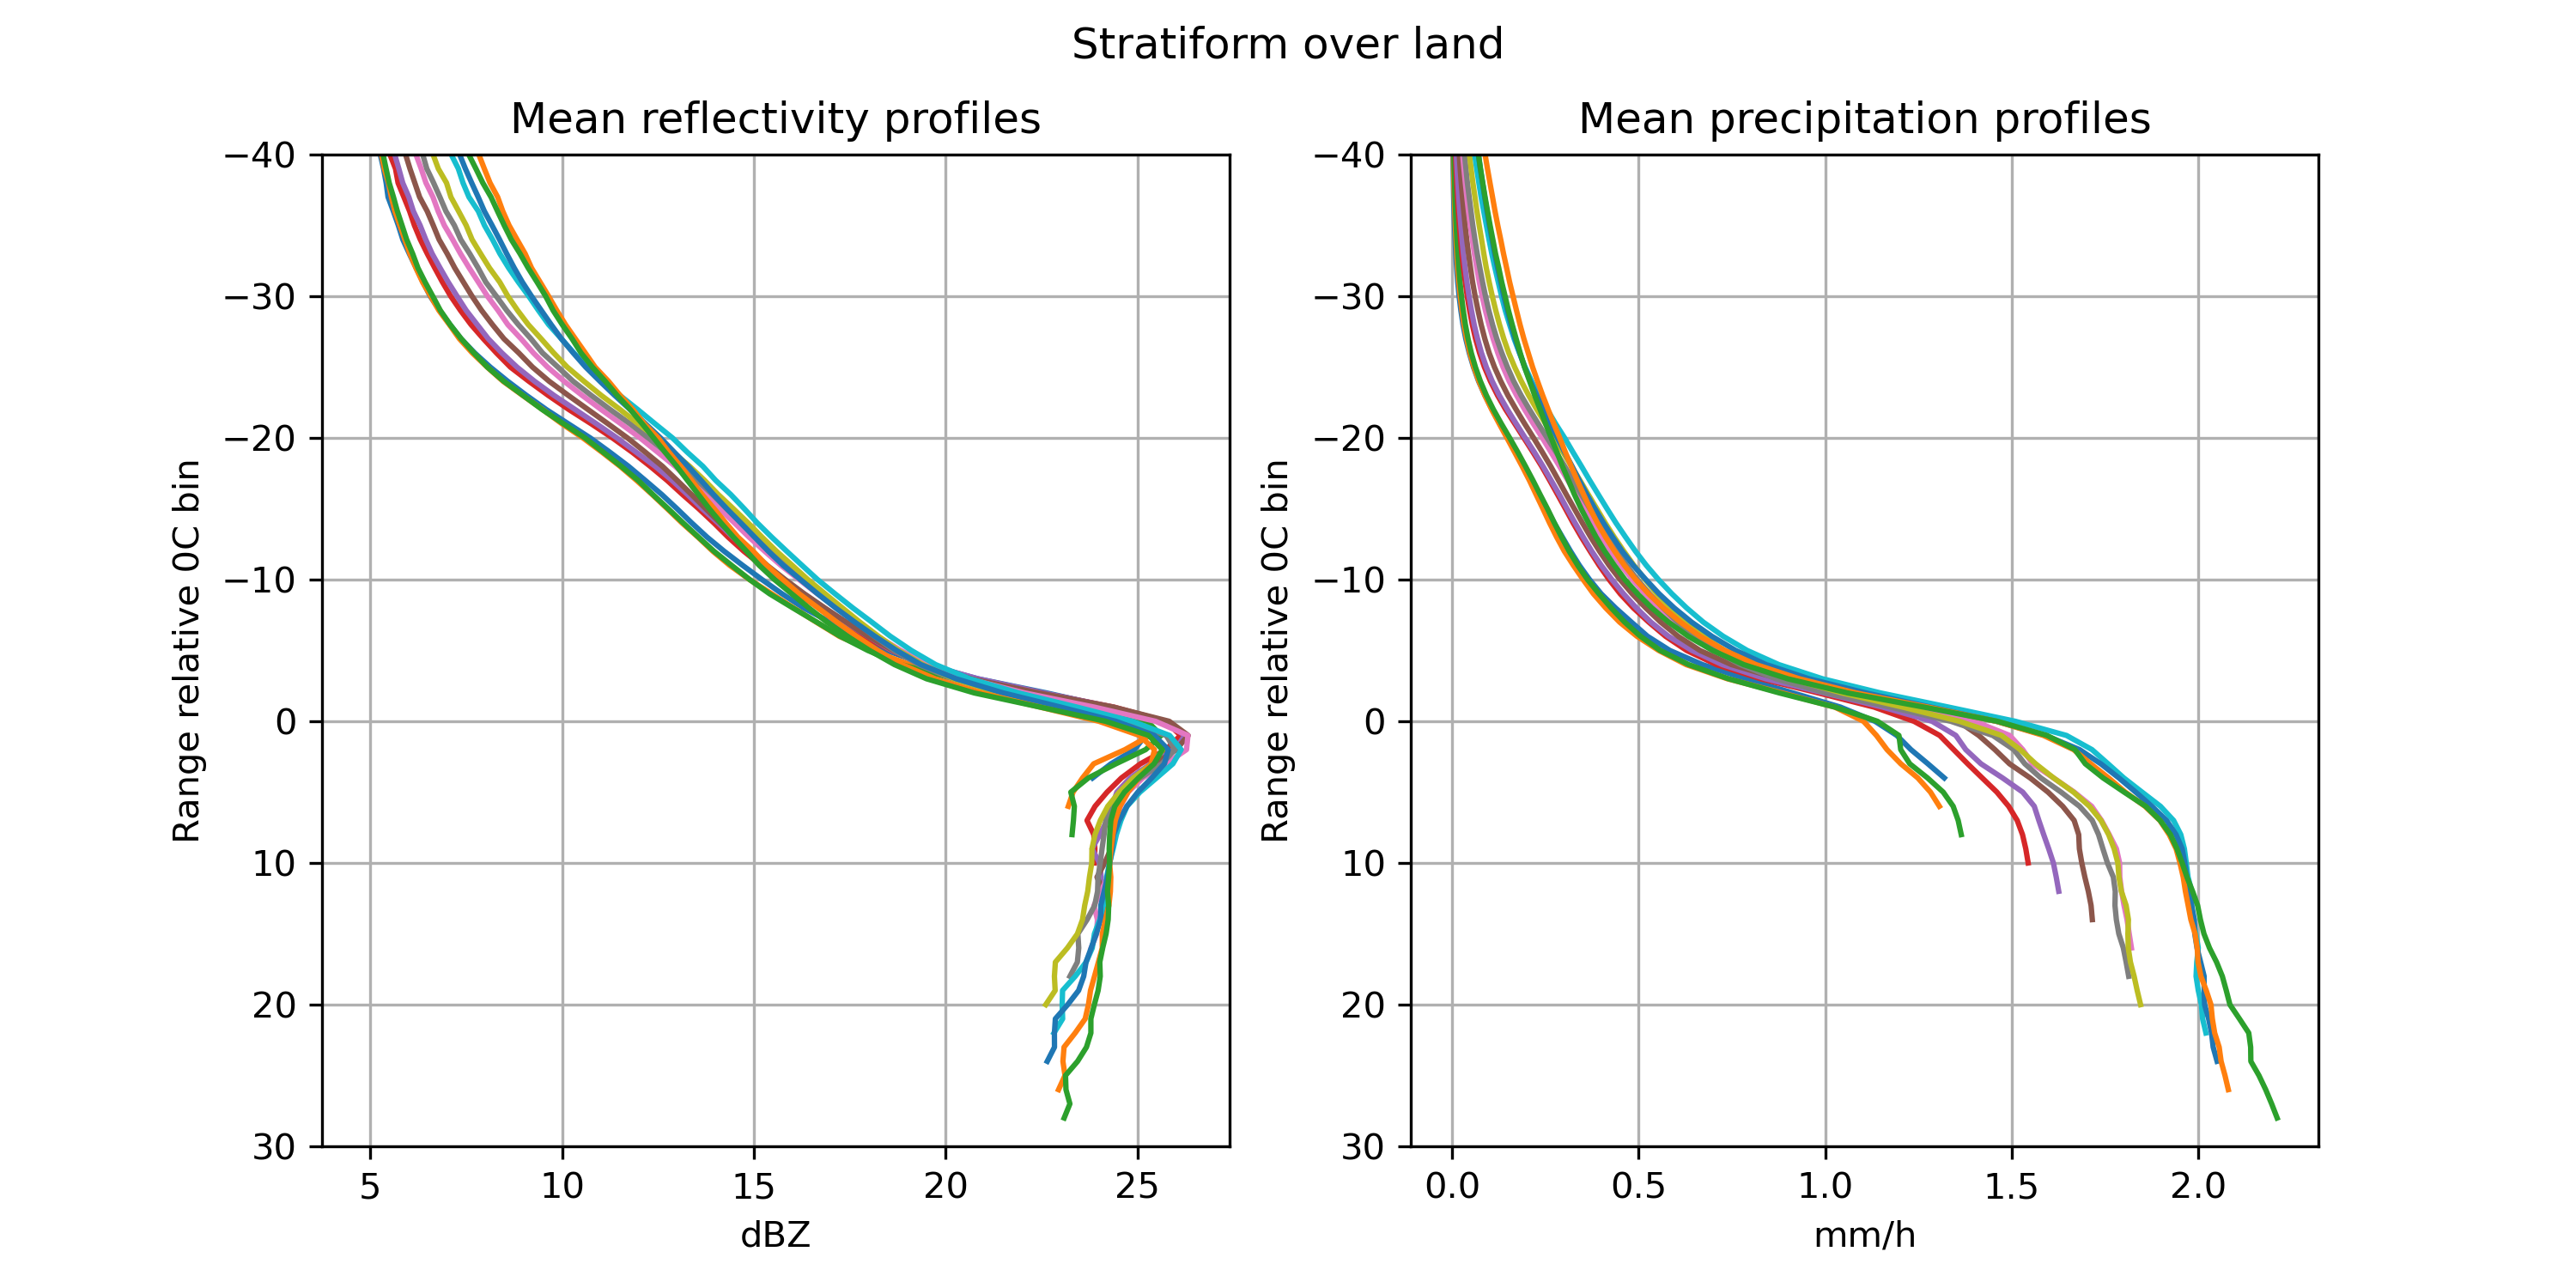
\includegraphics[width=0.85\textwidth]{reflectivityProfiles.png}
        \caption{Mean reflectivity and precipitation rate profiles}
        \label{fig:fig1}
    \end{figure}
\subsection*{Science Questions}   
    \begin{itemize}
    \item
      Can we derive DPR surface precipitation estimates more accurate than
      mean-profile-based extrapolations?
    \item
      Are the precipitation rate distributions below the freezing level
      unbiased? Given their impact on estimating the surface precipitation,
      this is an import question to address.
    \end{itemize}
    
    
\section*{Methodology}
\subsection*{Surface precipitation estimation}
    
The simplest method to estimate the precipitation rate at a given height
above the sea level from a precipitation rate at a higher level is to
rescale the higher level value by the ratio of the climatologic mean
precipitation rates at the two levels. Mathematically, this may be
written as
    
    \begin{equation}
    PR(H_1)=PR(H_2) \frac {<PR(H_1)>} {<PR(H_2)>} 
    \end{equation}

where $PR$ is the precipitation rate, $H_1$ is the height where the
estimate is needed, but for which no direct measurement is available,
$H_2$ is a height ($H_2>H_1$) where a radar
measurement is available, and operator $<\square>$ denotes the
climatologic mean over a large dataset characterized by the same
freezing level, surface and precipitation type.
    
While simple, the challenge in applying a clutter based correction
methodology based on Eq. (1) is the derivation of the correction factors
$\frac {<PR(H_1)>} {<PR(H_2)>}$ for all possible ($H_1$,$H_2$)
pairs. However, because the ground clutter depth is a function of the
scanning incidence angle, estimates of the climatologic correction
factor derived from near-nadir reflectivity observations and
precipitation estimates may be used to mitigate the clutter near the
edges of the swath. Moreover, because the mean reflectivity profiles
appear to be very similar when plotted relative to the 0C isotherm (Fig. 1), it may be postulated that 
$\frac {<PR(H_{1,0C})>} {<PR(H_{2,0C})>}$
is constant, where
($H_{1,0C},H_{2,0C}$) are heights ($H_1$,$H_2$) expressed
relative to the FL height.
    
The veracity of this hypothesis is tested, at the same time with the
effectiveness of the clutter correction, using near-nadir DPR
precipitation rate products. This is explained in the following
paragraphs.
    
Specifically, one year (i.e. 2018) of DPR observations is processed and
all reflectivity profiles over land characterized by fewer than eight
bins affected by clutter are selected. Additional variables such as the
associated precipitation type, the freezing level height and the
estimated precipitation rates are selected. The dataset is partitioned
based on the freezing level height in 12 distinct subsets, with the
freezing level heights of each subset within 125 m of 1.875+$k$*0.25
km with $k$ varying from 0 to 11. This dataset allows for both the
investigation of the postulated
$\frac {<PR(H_{1,0C})>} {<PR(H_{2,0C})>}$ invariance and the
effectiveness of various types of clutter mitigation including 
the one based on Eq. (1).
    
As $\frac {PR(H_1)} {PR(H_2)}$ may be significantly different from
the ratio of the climatologic rates for individual observations, it is
conceivable that a stratification of $\frac {<PR(H_1)>} {<PR(H_2)>}$
based on additional factors such as relative humidity, wind shear, etc.
improve the accuracy of the clutter correction. However, in practice,
these factors may not be estimated reliably either from the DPR
observations or from the NWP products associated with them. It is 
possible though that some of these factors have a distinctive signature
in the distribution of the observed reflectivity above the clutter. It
is therefore possible that a stratification of the observed reflectivity
profiles based on distinctive features such as gradients, magnitude, 
curvature, etc. may result in $\frac {<PR(H_1)>} {<PR(H_2)>}$
distributions different from that associated with the entire dataset. 
However, rather than subjectively formulating features and explicitly
stratifying the dataset and analyzing the resulting distributions, we
use a Machine Learning (ML) approach.  The ML approach does not require
the explicit of Eq. (1) and the stratification of the dataset. Instead,
it requires the organization of the dataset into a design matrix and a
response matrix \cite{bishop2006}. The design matrix is an array of 
reflectivity observations, with each row corresponding to a reflectivity
profile and each column to a reflectivity bin. The response matrix is an
array of precipitation rates, with each row corresponding to the
precipitation rate estimates associated 



\subsection*{Vertical distributions}
%% make 2x2 table
\begin{center}
\begin{figure}
\begin{tabular}{cc}
    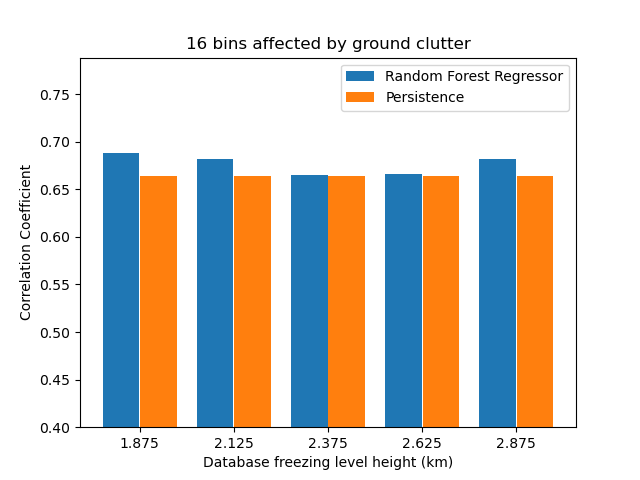
\includegraphics[width=0.495\textwidth]{Figs/corrCoeff_16bins.png}
    &
    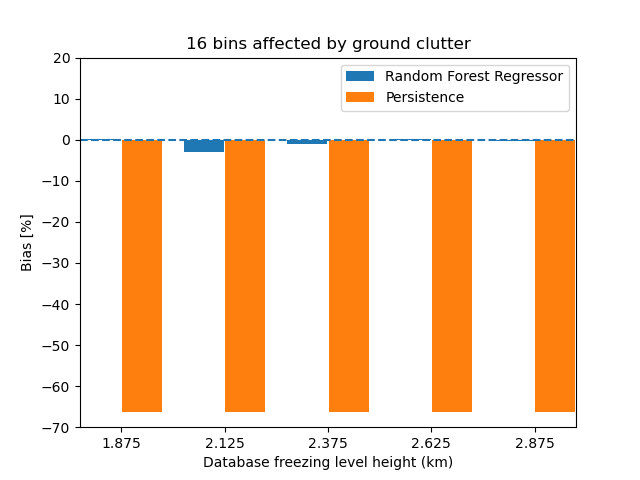
\includegraphics[width=0.495\textwidth]{Figs/bias_16bins.png}\\

    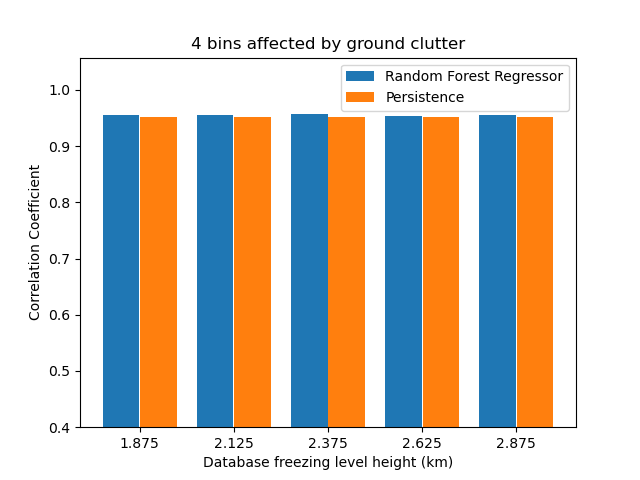
\includegraphics[width=0.495\textwidth]{Figs/corrCoeff_04bins.png}
    &
    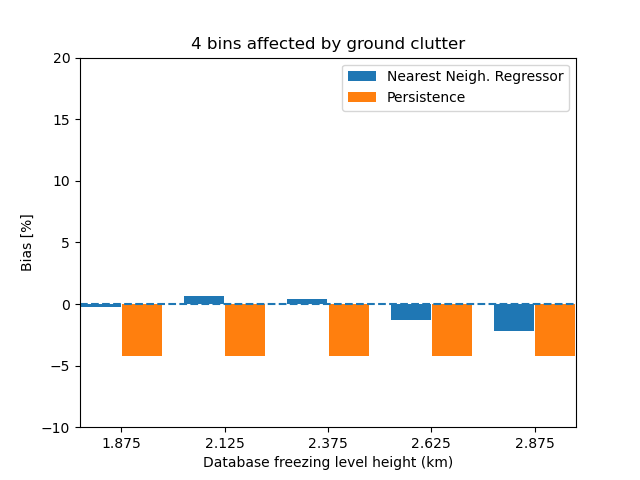
\includegraphics[width=0.495\textwidth]{Figs/bias_04bins.png}\\ 
\end{tabular}
\caption{Performance of a random forest based clutter correction method.}
\end{figure}
\end{center}
        
\bibliography{references}
\bibliographystyle{plain}
    
\end{document}